\section{Generating The Art}

After generating all the formulae to a particular size the next step in our algorithm is
to generate all the art corresponding to each formulae as depicted in the example seen
previously. Generating all the 2x2 formulae revealed some hidden structure to our results.

\subsection{All the 2x2 Art}
\begin{figure}
\begin{center}
\begin{tabular}{r c l}
Formulae & Level & Pictures \\
\tiny{none} & 0 & empty \\
\tiny{(true), (false)} & 1 &
    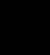
\includegraphics[width=.25in]{../presentation/2x2/Shape1LVL1.png}~
    
\includegraphics[width=.25in]{../presentation/2x2/Shape2LVL1.png} \\
\tiny{none} & 2 & empty \\
\tiny{($<$ x 1), ($<$ y 1), ($<$ x y), ($<$ 0 x), ($<$ 0 y), ($<$ y x)} & 3 & 
    
\includegraphics[width=.25in]{../presentation/2x2/Shape1LVL3.png}~
    
\includegraphics[width=.25in]{../presentation/2x2/Shape2LVL3.png}~
    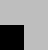
\includegraphics[width=.25in]{../presentation/2x2/Shape5LVL3.png}~
    
\includegraphics[width=.25in]{../presentation/2x2/Shape6LVL3.png}~
    
\includegraphics[width=.25in]{../presentation/2x2/Shape3LVL3.png}~
    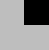
\includegraphics[width=.25in]{../presentation/2x2/Shape4LVL3.png}\\
\tiny{(not ($<$ x y)), (not ($<$ y x))} & 4 & 
    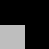
\includegraphics[width=.25in]{../presentation/2x2/Shape2LVL4.png}~
    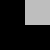
\includegraphics[width=.25in]{../presentation/2x2/Shape1LVL4.png} \\
\tiny{($<$ (y + x) 1), ($<$ (y * x) 1), ($<$ 0 (y + x)), ($<$ 1 (y + x))} & 5 & 
    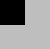
\includegraphics[width=.25in]{../presentation/2x2/Shape2LVL5.png}~
    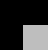
\includegraphics[width=.25in]{../presentation/2x2/Shape1LVL5.png}~
    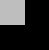
\includegraphics[width=.25in]{../presentation/2x2/Shape3LVL5.png}~
    
\includegraphics[width=.25in]{../presentation/2x2/Shape4LVL5.png} \\
\tiny{none} & 6 & empty \\
\tiny{(or ($<$ y  x) ($<$ x  y))} & 7 &
    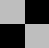
\includegraphics[width=.25in]{../presentation/2x2/Shape1LVL7.png}\\
\tiny{(not (or ($<$ y  x) ($<$ x  y)))} & 8 &
    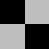
\includegraphics[width=.25in]{../presentation/2x2/Shape1LVL8.png}
\end{tabular}
\end{center}

\caption{All the 2x2 art with its corresponding complexity.}
\label{fig:2x2}
\end{figure}

From Figure~\ref{fig:2x2}, some things are immediately obvious.  First of all,
as might match one's intuition, the all-black and all-white pictures are the
least complex pictures.  Secondly, one can see that if a formula of size $n$
exists to create a certain picture, then that picture's inverse has a
complexity of one of $n-1$, $n$, or $n+1$.  Examples of this last phenomenon
can be seen between rows 7 and 8, as well as between rows 3 and 4.  This occurs
for the simple reason that adding one symbol ({\tt not}) creates a picture's
inverse.  Also, somewhat intriguingly, we can see gaps at 2 and 6.  Although
there are formulae of size 2, none of those formulae produce a picture that has
not been already produced by formulae of a smaller size e.g (not true) , (not false).


The natural extension of our exploration of all the 2x2 artwork and the structure within the set of 2x2 artwork as a whole is the following question. What is the correlation between visual complexity (an inherently subjective notion) and
Formula complexity?  

\section{Assessing Formula Complexity}
Formula complexity is a ``low-powered'' version of Kolmogorov Complexity.  KC
allows the full power of a programming language to be put to bear in describing
how an output is produced.  In particular, KC allows for the definition and
application of functions as well as conditional statements.  In our language,
the only things which can be used are formulae with a boolean result
involving only the logical atoms {\tt and}, {\tt or}, {\tt not}, {\tt true},
and {\tt false}, as well as the numerical atoms of {\tt 0}, {\tt 1}, {\tt x},
{\tt y}, {\tt +}, {\tt *}, and {\tt <}.

Because formula complexity disallows loops and function definitions, every
formula represents a terminating program.  Even more, since the domain of all
of the operators is total, this means that every well-typed formula represents
a non-crashing program\footnote{This is why the division and modulous operators
were excluded, as {\tt 12 mod 0} and {\tt 12 / 0} result in a crashing program
rather than a value.}.  Thus, in exchange for ``powering down'' KC, we can
actually enumerate and test all formulae, without worrying about infinite loops
or crashes.



Formula complexity is an inherent attribute of an output. 
It is defined as the size of the smallest formula able to produce the output in question. 

% Say how we produce an output from a formula

Producing an output from a formula starts with generating the formula in python. After
that python transfers the formula to racket and performs a number of translations on the original formula in
order to produce the final output.
The final output consists of a pattern a program and a complexity.
The pattern is the pictorial output.
The program is the formula that we started with.
The complexity (formula) is the record of the smallest possible formula size that could produce the pictorial output.

